\section{坐标轴}

\subsection{类型简介}

坐标轴,是可视化图表中经常出现的一种图形,由轴线、刻度和标签组成,可以分为水平的x轴和垂直方向上的y轴。D3 支持了以下四种绘制坐标轴的函数,使用起来很方便。

\begin{enumerate}
    \item \verb|d3.axisTop()|:创建顶部坐标轴
    \item \verb|d3.axisRight()|:创建垂直居右坐标轴
    \item \verb|d3.axisBottom()|:创建底部坐标轴
    \item \verb|d3.axisLeft()|:创建垂直居左坐标轴
\end{enumerate}

\subsection{x轴坐标轴}

\begin{minted}[frame=lines,framesep=2mm,baselinestretch=1.2,fontsize=\footnotesize,linenos]{html}
<script>
  // 将 SVG 画布的宽高定义成变量
  var width = 400,
    height = 100;

  // 需要刻画的数据
  var data = [10, 15, 20, 25, 30];

  // 添加 SVG 画布
  var svg = d3
    .select("body")
    .append("svg")
    .attr("width", width)
    .attr("height", height);

  // 创建线性比例尺
  // 设置其宽高、定义域值域
  // 从定义域到值域:10->0,30->300
  var scale = d3
    .scaleLinear()
    .domain([d3.min(data), d3.max(data)])
    .range([0, width - 100]);

  // 创建横向底部的x轴,并向x轴添加比例尺
  var x_axis = d3.axisBottom().scale(scale);

  // 创建“组”并向其中插入x轴坐标
  svg.append("g").call(x_axis);
</script>
\end{minted}

运行这个例子,可以观察到已作出了一个x轴坐标轴。如\figref{fig:axis_x}为其渲染出的形状。

\begin{figure}[htbp]
    \centering
    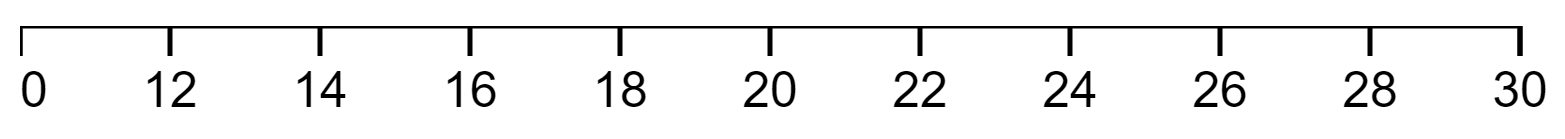
\includegraphics[width=0.6\textwidth]{figure/D3/axis_x.png}
    \caption{\textbf{D3中绘制x轴坐标轴}}
    \label{fig:axis_x}
\end{figure}

对应生成的HTML代码如下:

\begin{minted}[frame=lines,framesep=2mm,baselinestretch=1.2,fontsize=\footnotesize,linenos]{html}
<svg width="400" height="100">
  <g fill="none" font-size="10" font-family="sans-serif" text-anchor="middle">
    <path class="domain" stroke="currentColor" d="M0,6V0H300V6"></path>
    <g class="tick" opacity="1" transform="translate(0,0)">
      <line stroke="currentColor" y2="6"></line>
      <text fill="currentColor" y="9" dy="0.71em">10</text>
    </g>
    <g class="tick" opacity="1" transform="translate(30,0)">
      <line stroke="currentColor" y2="6"></line>
      <text fill="currentColor" y="9" dy="0.71em">12</text>
    </g>
    ...
  </g>
</svg>
\end{minted}

\subsection{y轴坐标轴}

类似地,我们也可以创建垂直方向上的轴,代码如下:

\begin{minted}[frame=lines,framesep=2mm,baselinestretch=1.2,fontsize=\footnotesize,linenos]{html}
<script>
  var width = 400,
    height = 400;

  var data = [10, 15, 20, 25, 30];
  var svg = d3
    .select("body")
    .append("svg")
    .attr("width", width)
    .attr("height", height);

  var scale = d3
    .scaleLinear()
    .domain([d3.min(data), d3.max(data)])
    .range([height / 2, 0]);

  var y_axis = d3.axisLeft().scale(scale);

  svg.append("g").attr("transform", "translate(50, 10)").call(y_axis);
  // translate transform 操作调整了坐标轴在SVG图中的位置
</script>
\end{minted}

运行后的效果如\figref{fig:axis_y}所示。

\begin{figure}[htbp]
    \centering
    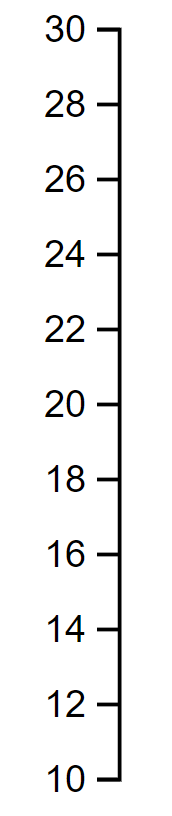
\includegraphics[width=0.1\textwidth]{figure/D3/axis_y.png}
    \caption{\textbf{D3中绘制y轴坐标轴}}
    \label{fig:axis_y}
\end{figure}

\subsection{同时包含x轴和y轴坐标轴}

现在我们可以把x轴和y轴并在一张图里,代码如下,效果见\figref{fig:axis_xy}所示。

\begin{minted}[frame=lines,framesep=2mm,baselinestretch=1.2,fontsize=\footnotesize,linenos]{html}
<script>
  var width = 400,
    height = 400;
  var data = [10, 15, 20, 25, 30];

  var svg = d3
    .select("body")
    .append("svg")
    .attr("width", width)
    .attr("height", height);

  var xscale = d3
    .scaleLinear()
    .domain([0, d3.max(data)])
    .range([0, width - 100]);

  var yscale = d3
    .scaleLinear()
    .domain([0, d3.max(data)])
    .range([height / 2, 0]);

  var x_axis = d3.axisBottom().scale(xscale);

  var y_axis = d3.axisLeft().scale(yscale);

  svg.append("g").attr("transform", "translate(50, 10)").call(y_axis);

  var xAxisTranslate = height / 2 + 10;

  svg
    .append("g")
    .attr("transform", "translate(50, " + xAxisTranslate + ")")
    .call(x_axis);
</script>
\end{minted}

\begin{figure}[htbp]
    \centering
    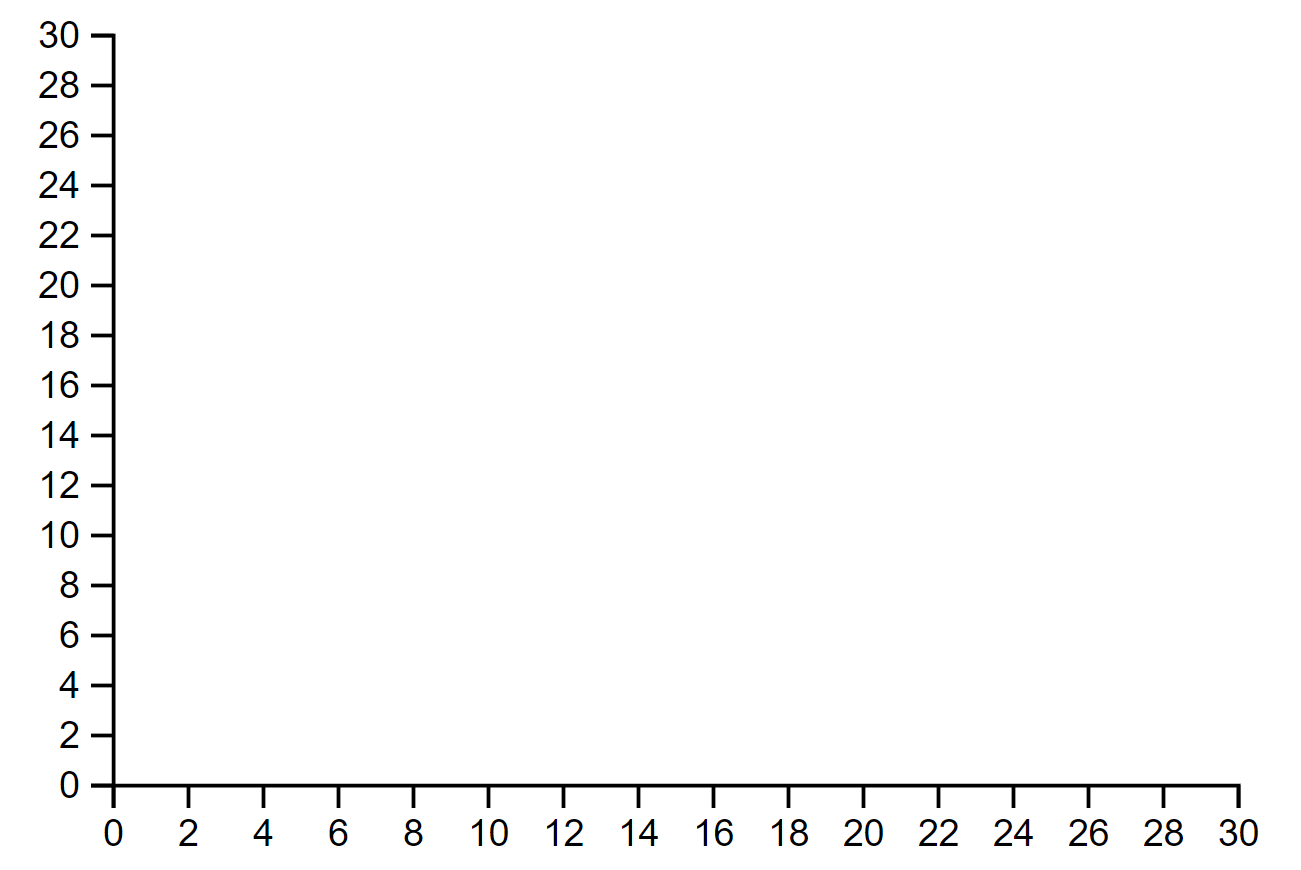
\includegraphics[width=0.6\textwidth]{figure/D3/axis_xy.png}
    \caption{\textbf{D3中同时绘制出x轴和y轴坐标轴}}
    \label{fig:axis_xy}
\end{figure}